\section{Parsing}
\label{sec:parsing}

Il formato DXF organizza il disegno in primitive geometriche: \texttt{LINE}, \texttt{POLYLINE}, \texttt{ARC}, \texttt{CIRCLE}, ecc. Queste entità sono raggruppate in layer, che consentono di separare logicamente i diversi elementi del disegno (ad esempio muri, porte, finestre, arredi, testo). Oltre ai layer, il formato DXF supporta i blocchi (\texttt{BLOCK}), componenti riutilizzabili comunemente impiegati per rappresentare porte e finestre. Un blocco viene definito una volta all'interno del file e può essere istanziato più volte tramite entità \texttt{INSERT}, ciascuna con una propria posizione, scala e rotazione: questa funzionalità è particolarmente utile per rappresentare elementi ripetuti, come porte, finestre o arredi, che compaiono più volte nella stessa planimetria.

L'obiettivo della fase di parsing è estrarre da queste primitive le informazioni geometriche necessarie alla costruzione della mesh, collassando tutte le primitive sotto forma di segmenti, così da ottenere una rappresentazione uniforme.

Si consideri il modello CAD corretto durante il preprocessing (Sezione \ref{sec:preprocessing}), che presenta layer standardizzati (\texttt{A-WALL}, \texttt{A-DOOR}, \texttt{A-WINDOW}) e blocchi rinominati (\texttt{BLOCK-DOOR-1}, \texttt{BLOCK-WINDOW-1}, \ldots, \texttt{BLOCK-WINDOW-4}).

Il parsing viene realizzato in C++ mediante la libreria libdxfrw \cite{libdxfrw}, che fornisce un'interfaccia per la lettura dei file DXF. Si definisce anzitutto la struttura di un segmento (Figura~\ref{fig:segment-uml}), rappresentato come coppia di vertici (posizioni nello spazio) e un tag che ne indica la semantica (muro, porta o finestra):
\begin{figure}[H]
	\centering
	\begin{tikzpicture}
	\begin{class}[text width=3.5cm]{SegmentLayer}{0,0}
		\operation{<<enumeration>>}
		\attribute{Wall}
		\attribute{Window}
		\attribute{Door}
	\end{class}
	
	\begin{class}[text width=5cm]{Segment}{6,0}
		\attribute{+ start : Point}
		\attribute{+ end : Point}
		\attribute{+ layer : SegmentLayer}
	\end{class}
	\end{tikzpicture}
	
	\caption{Diagramma UML delle entità \texttt{Segment} e \texttt{SegmentLayer}, che rappresentano rispettivamente un segmento geometrico e la sua semantica (muro, porta o finestra).}
	\label{fig:segment-uml}
\end{figure}


Questa classificazione per layer e per blocco è fondamentale perché, come si vedrà successivamente, consente di trattare in modo differenziato muri, porte e finestre durante la fase di estrusione. La classe del parser (Figura~\ref{fig:drwparser-uml}) implementa le callback necessarie per gestire i diversi tipi di entità:
\begin{figure}[H]
	\centering
	\begin{tikzpicture}
		\begin{class}[text width=12cm]{DRWParser}{0,0}
	 		\attribute{- walls : Segment [*]}
			\attribute{- doors : Segment [*]}
			\attribute{- windows : Segment [*]}
			\operation{+ addLine(data : DRW\_Line) : void}
			\operation{+ addLWPolyline(data : DRW\_LWPolyline) : void}
			\operation{+ addArc(data : DRW\_Arc) : void}
			\operation{+ addInsert(data : DRW\_Insert) : void}
			\operation{+ addBlock(data : DRW\_Block) : void}
			\operation{+ endBlock() : void}
			\operation{+ classifyLayer(name : String) : SegmentLayer}
		\end{class}
	\end{tikzpicture}
	\caption{Diagramma UML della classe \texttt{DRWParser}.}
	\label{fig:drwparser-uml}
\end{figure}


Tra le callback messe a disposizione, quelle di maggiore interesse sono:
\begin{itemize}
	\item \texttt{addLine()}: viene invocata per ogni segmento (\texttt{LINE}) presente nel disegno. I due punti estremi vengono memorizzati direttamente come segmento;
	
	\item \texttt{addLWPolyline()}: per le polilinee (\texttt{LWPolyline}), si iterano i vertici della polilinea per generare una sequenza di segmenti consecutivi;
	
	\item \texttt{addArc()}: per gli archi (\texttt{ARC}), si estraggono il raggio, il punto base, l'angolo iniziale e l'angolo finale; a partire da questi dati si calcolano i due punti estremi dell'arco, corrispondenti agli spigoli delle pareti adiacenti, e il segmento che li collega costituisce la rappresentazione della porta;
	
	\item \texttt{addInsert()}, \texttt{addBlock()}: gestiscono le istanze dei blocchi. Poiché le primitive all'interno di un blocco sono definite in coordinate locali, è necessario applicare una trasformazione (posizione, scala, rotazione) per riportarle in world space.
\end{itemize}

Per distinguere i segmenti in base alla loro semantica si utilizza il nome del layer ((Algoritmo~\ref{alg:classify_layer})):
\begin{algorithm}[htbp]
	\begin{algorithmic}[1]
		\Function{ClassifyLayer}{$name$}
		\If{$name = \texttt{"A-DOOR"}$}
		\State \Return \textsc{Door}
		\ElsIf{$name = \texttt{"A-WALL"}$}
		\State \Return \textsc{Wall}
		\ElsIf{$name = \texttt{"A-WINDOW"}$}
		\State \Return \textsc{Window}
		\Else
		\State \Return \textsc{None}
		\EndIf
		\EndFunction
	\end{algorithmic}
	
	\caption{Classificazione del layer di un segmento}
	\label{alg:classify_layer}
\end{algorithm}


La stessa logica di corrispondenza per nome viene applicata al riconoscimento dei blocchi (\texttt{BLOCK-DOOR}, \texttt{BLOCK-WINDOW}) all'interno di \texttt{addBlock()}; proprio per questo motivo, rinominare correttamente layer e blocchi durante il preprocessing è un passaggio imprescindibile per la corretta riuscita del parsing.

Al termine di questa fase si ottengono tre vettori, contenenti rispettivamente le primitive (sotto forma di segmenti) relative a muri, porte e finestre.

Per verificare la correttezza del parsing si utilizza uno script Python che effettua il plot dei segmenti estratti (Figura ~\ref{fig:parsing}).
\begin{figure}[htbp]
	\centering
	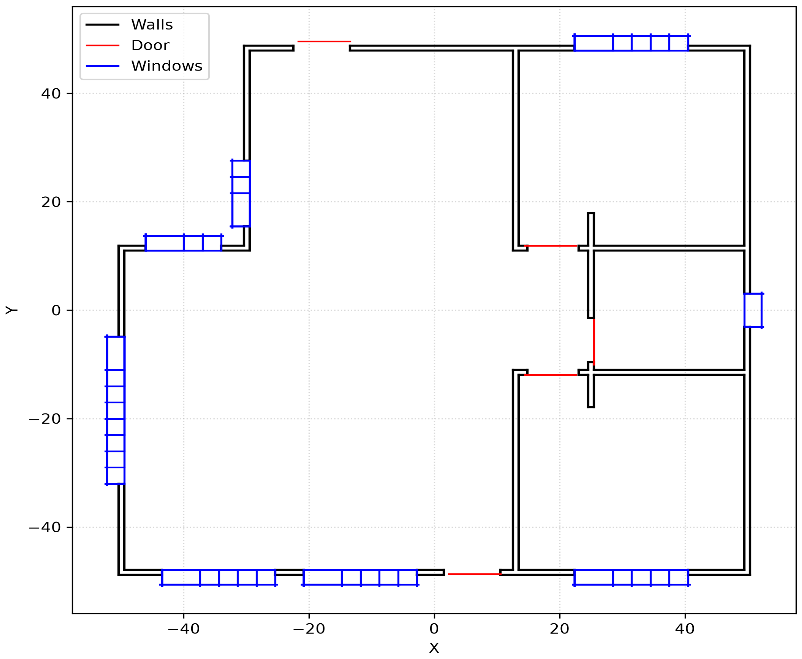
\includegraphics[width=1\textwidth]{figures/3_progettazione_pipeline/parsing.png}
	\caption{Risultato del parsing: le primitive geometriche estratte dal file DXF sono state collassate in segmenti e visualizzate tramite uno script Python per verificarne la correttezza.}
	\label{fig:parsing}
\end{figure}